%!TEX root = ../MasterThesis.tex

\section{Existing System Design Approaches}
\label{sec:system_approaches}

When trying to solve issues of information integration between organisations there are already existing solutions, that have to be examined whether they might fit the \gls{E-commerce} fraud investigation scenario or not.

\subsection{The \gls{ETL} processes}
\label{subsec:etl_process}

To begin with, retrieving, transforming and combining data from multiple dispersed data sources is not a completely new problem, and is actually part of ``Extract-Transform-Load'' or \gls{ETL} processes within an organisation. The basic idea is the same as in the concept shown in this thesis; namely to get as much information as possible from the various databases, that are in use within a company, harmonize (aka transform) the information from each of them into a shared data model, and use the cleaned up and combined information repository for doing advanced business analytics and predictions. Data within an organisation is created and maintained by different business-related tools. Each of these will store the information into their own database using a vendor-specific schema. Other business-relevant data might be stored in structured files sometimes using a proprietary format, such as Excel files. Each of these data sources have to be accessed, the valuable information have to be extracted and mapped against each other, before the analysis of it can begin on a separate data store, that holds the combined data set. The whole process is visualized in Figure~\ref{fig:images_etl_process}. \\

\begin{figure}[!ht]
  \centering
  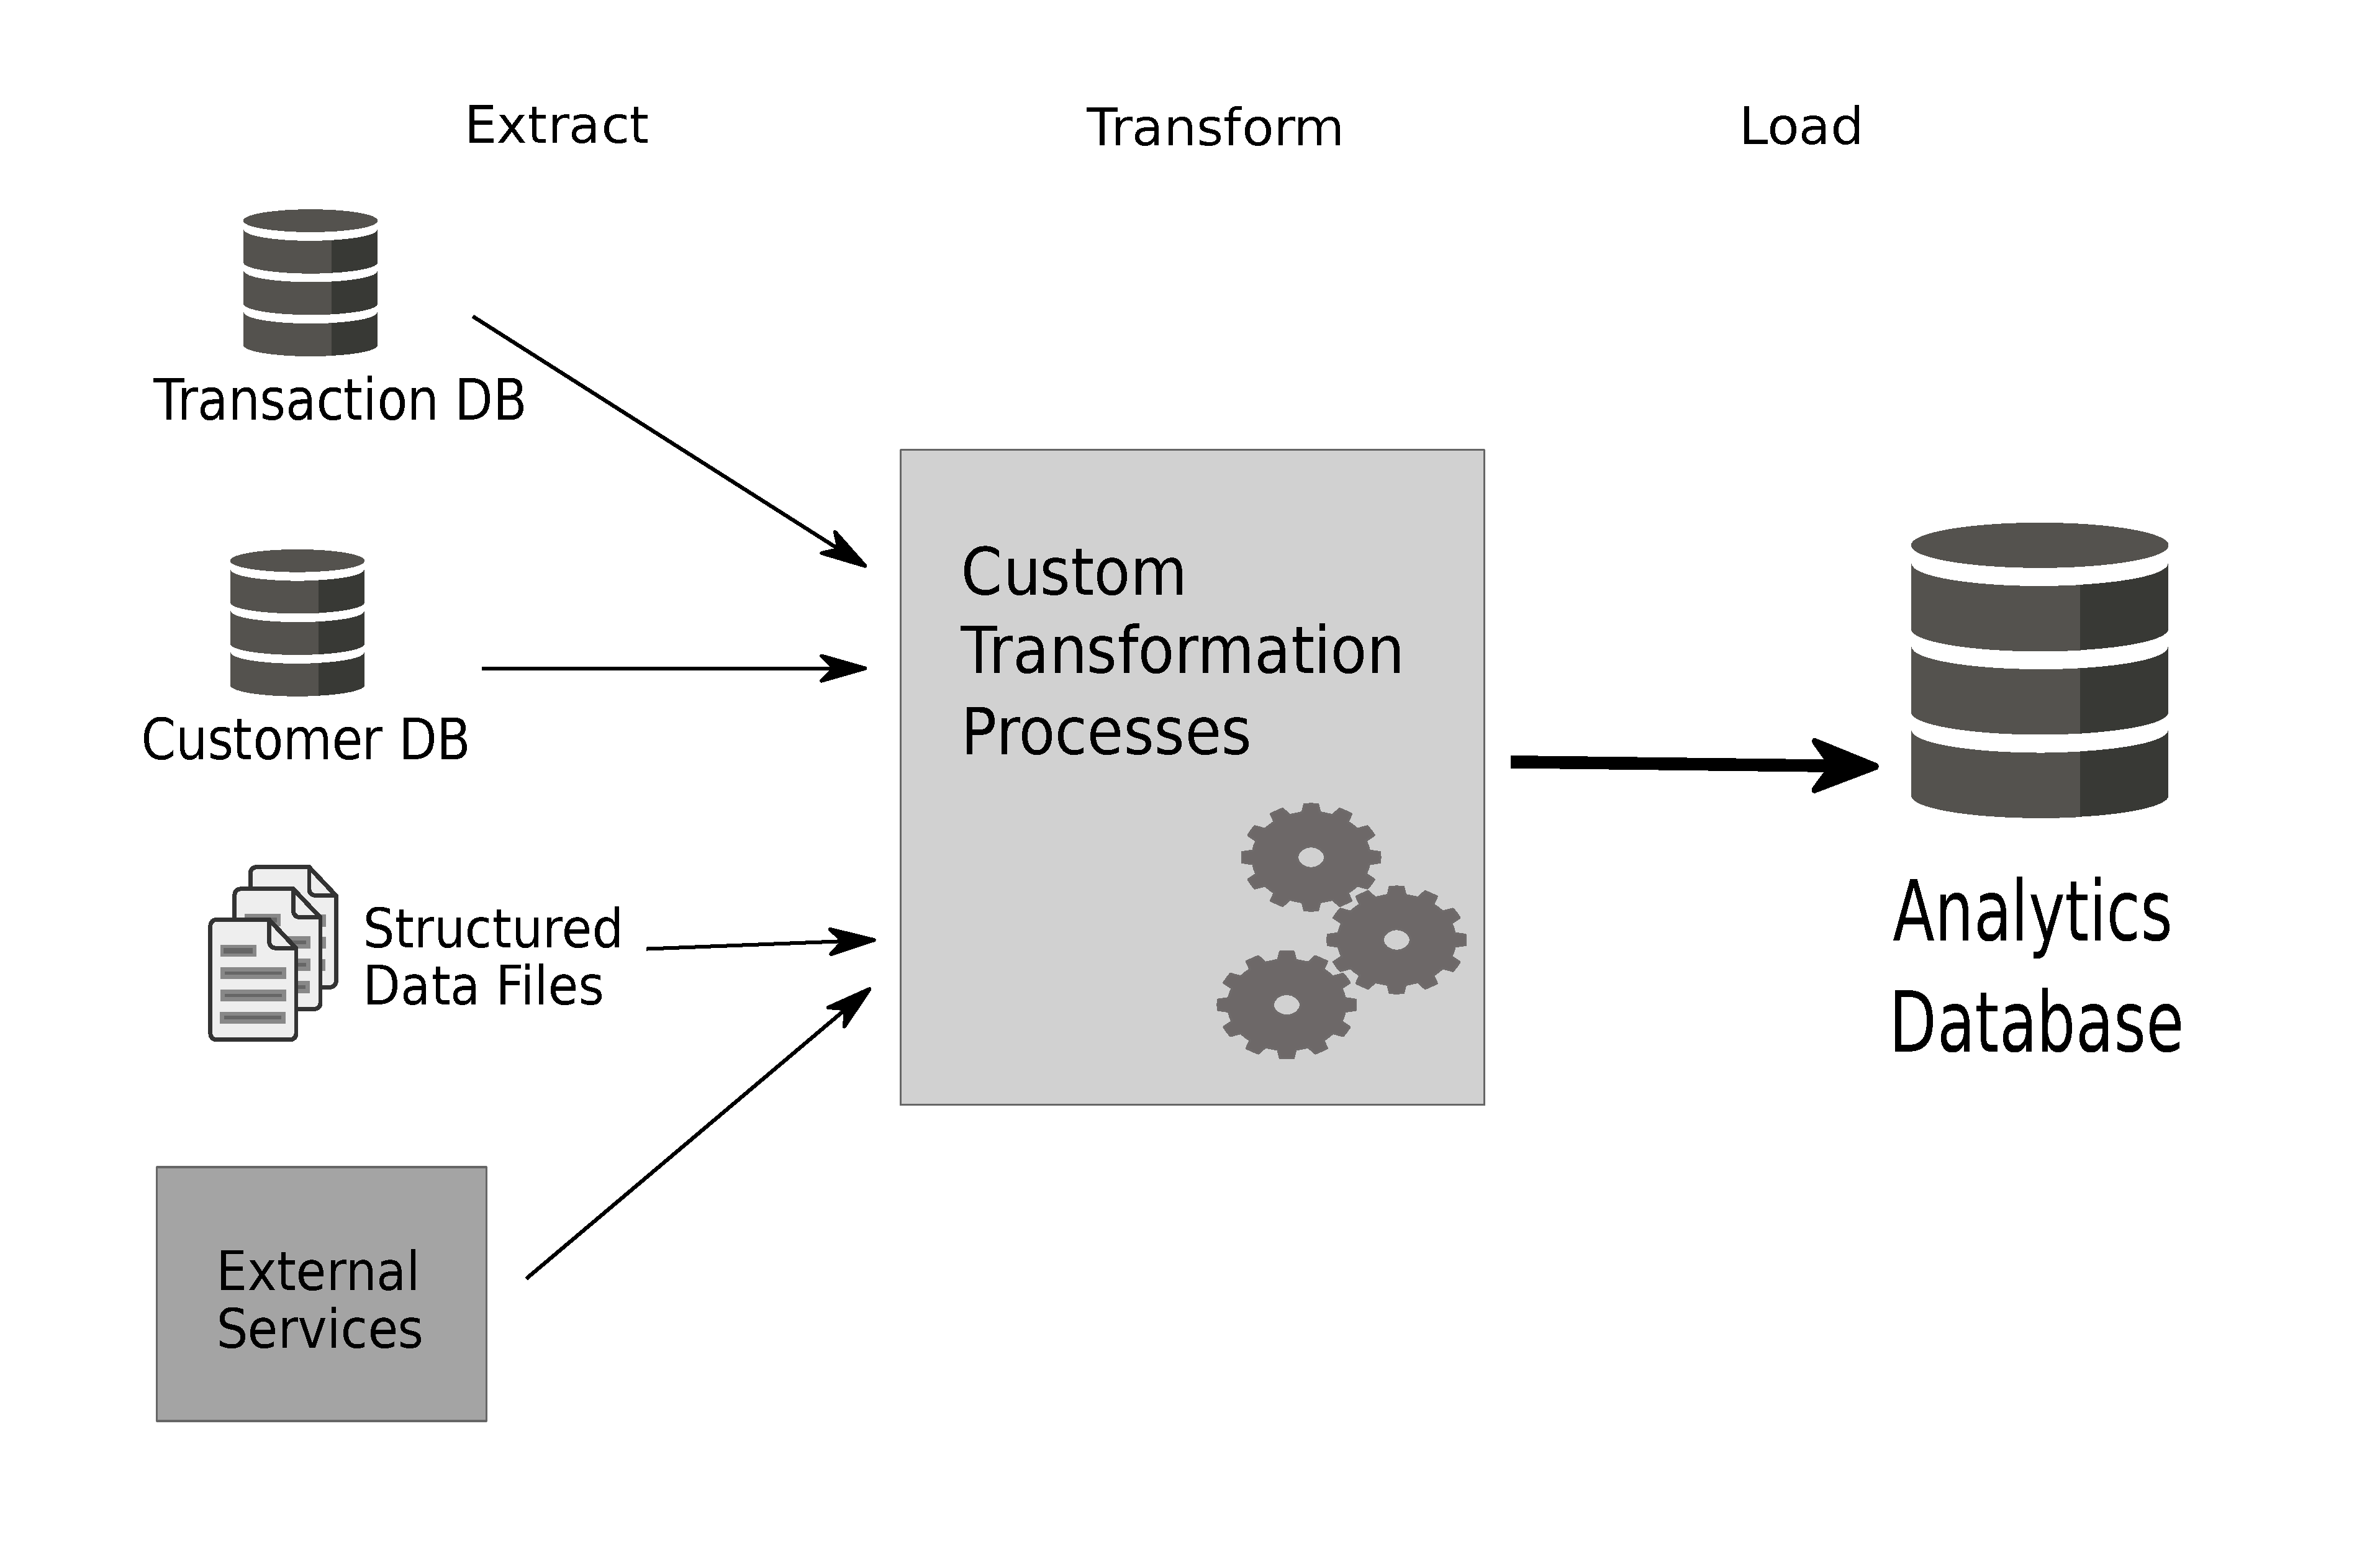
\includegraphics[width=0.9\columnwidth]{images/etl_process.pdf}
  \caption{\gls{ETL} process within a company \citep[pg. 165]{wood2014linked}}
\label{fig:images_etl_process}
\end{figure}

Still these \gls{ETL} processes rely on an in-depth knowledge of the data structures, that are used in each of the information sources as well as require a direct access to the databases and files for retrieving the information. Although these conditions are not cumbersome to work with within an organisation, they will be a real show stopper if one has to integrate data sources across company boundaries. As the integration of the information takes place on the database level, allowing external access to your internal databases will not only open up access to your business internals, but will also make it more complicated to change the underlying database structure and software. Any changes to one of these require a negotiation between the owner of the data source and all of the external partners attached to it. \\

Beside this obviously limited usage for the \gls{E-commerce} fraud investigation scenario at the whole, one can assume that these \gls{ETL} processes are still in use for operating the daily business of each stakeholder. They can be helpful at a later point in the discussion, when a decision has to be made about how a stakeholder can prepare and transform his internal data resources for external consumptions.

% section etl_process

\subsection{Web Services}
\label{subsec:web_services}

With the development of the \gls{E-commerce} scenario there was also a need to integrate business functionalities from various service providers, whose are operating on the Internet. Valid examples for this kind of integration are the usage of the \gls{PSP} for doing the payment as well as the \gls{LSP} for handling the shipping process. These approaches resulted in the ``Service Oriented Architecture'' paradigm, that enables application services provided by different vendors to talk to each other via a public facing programming interface (aka \gls{API}). The only requirement for such interoperability to work properly is, that each public interface follows some standardised or commonly agreed upon guidelines to be vendor-, platform- as well as language-agnostic. One possible implementation of these concepts are the so-called Web Services, that use the WS* protocols and standards from the \gls{W3C} with the extensible markup language (aka \gls{XML}) and the \gls{HTTP} protocol at their core \citep{josuttis2007soa}. \\

Like the \gls{HTML} format, that is used to represent Web pages on the Internet, \gls{XML} is originally based on \gls{SGML}, but instead of formalising markup tags for structuring and styling textual content it is a meta-language allowing everyone to define his or her own markup languages. In this matter it doesn’t dictate what tags are available to structure the information; instead it includes some basic guidelines for creating wellformed and valid documents that uses domain-specific tags, which can be freely defined and structured by the creator of the \gls{XML} document. Therefore it is better suited in situations, in which a computer has to parse and evaluate the content of a message; assuming the computer program knows the structure of the message. \\

In an additional step the author of the \gls{API} could also specify an \gls{XML} schema for each message, which describes the structure of the message with all the possible elements, their ordering, nesting level and data types in detail. By doing so the \gls{XML} parser program can later verify the content of a retrieved message against the \gls{XML} schema and check if it is a valid document related to the schema definition. \gls{XML} schematas are also expressed in \gls{XML} format and have been standardised by the \gls{W3C}. Being able to create custom markup languages via \gls{XML} has a huge benefit for machine-to-machine communication and is the basis for integrating Web Services (via the WS* protocols), but it still has limitations when it comes to figure out the semantics of those \gls{XML} messages. This is mostly due to the fact that each \gls{XML} document represents a new markup language and needs a specific \gls{XML} parser to be understood by the machine; also to distinguish commonly used tag names in an \gls{XML} document the creator has to place them into specific namespaces (aka \gls{XML} namespaces). But those \gls{XML} namespaces further complicate the automatic processing of \gls{XML} documents and increases the necessity to have custom instances of \gls{XML} parsers for each \gls{XML} document \citep{taylor2008p2p}. \\

An integration of information exchange via Web Services is usually handled separately for each Web Service interface. Looking at the payment service integration as \textbf{\underline{one}} possible example, the following steps are neccessary to allow a merchant to interact with the Web Service of a \gls{PSP}: \@

\begin{itemize}
  \item the \gls{PSP} has to define an interface (aka \gls{API}) that a merchant can use to exchange information with them
  \item the \gls{API} includes a set of data exchange messages, usually in \gls{XML} format, as well as a list of operations, that the interface supports
  \item the \gls{PSP} has to document each of these messages and operations, incl.\ their intended structures and semantics
  \item the \gls{PSP} has to provide access to the \gls{API} via an \gls{HTTP} endpoint running on a server at a specific \gls{URL}
  \item the \gls{PSP} usually restricts access to this interface for registered partners only; for this they have to provide a registration and identification mechanism
  \item the merchant has to register with the \gls{PSP} to be able to call into their Web Service \gls{API}
  \item the merchant receives some kind of token, that they can use to identify themselves with the Web Service later
  \item the merchant has to implement an \gls{API}-specific client-side wrapper, that knows how to talk to the interface; incl.\ calling one of the available operations as well as serializing and deserializing the messages between the Web Service and the client program
  \item the client program has to understand the structure and semantic of the messages exchanged with the Web Service
\end{itemize}

Although other merchants, that want to use the same \gls{API} from the \gls{PSP}, can use the same client-side wrapper (sometimes also provided by the \gls{PSP} for convenience) to send messages to this specific Web Service, they still have to make the \gls{API}-specific integration into their own Web shop. To be able to share more information with the \gls{PSP}, the merchant has to do likewise and provide an own \gls{API} for others to use to query for information (following the same steps as mentioned above). \\

Also, as the structures and semantics of the messages and operations of each Web Service interface are not standardized, integrating with another \gls{PSP} or merchant results in doing the same integration steps again and again. To make things worse, the mapping of the information coming from different \gls{API}s has to be implemented by the client, who wants to analyze the combined data set.   It soon becomes clear, that these necessary tasks will increase the time and effort with each additional stakeholder, who wants to participate in the collaborative system. \\

As conclusion one could easily see that integrating information between a larger group of participants is very limited with the existing Web Services approach. The steps neccessary for exchanging information result in huge efforts on all participating parties. As there is no common way to access and combine the information from each one of the participants, beside using the fundamental \gls{HTTP} protocol and \gls{XML} data format, there have to be a lot of collaborative work between each of them upfront, to come up with an approach to integrate the available \gls{API}s, and provide the rules for combining the different data structures.

% subsection web_services (end)

\subsection{Semantic Web}
\label{subsec:web_data}

``The Web is full of intelligent applications, with new innovations coming every day'' \citep{allemang2011semantic}. But each of those intelligent Web applications is driven by the data available to them. Data that is likely coming from different places in the global information space — accessible usually via a custom API on the server hosting those resources (see Section~\ref{subsec:web_services}). The more consistent the data available to the smart Web application is the better the service and its result will be. But to support an integration of the data from various Web services the semantics of the information delivered by each service has to be available — and there has to be a generalised, formalised way to express the semantic of that data. The focus on a standard that allows Web services to express the semantics of the data they provide also allows for global scalability, openness and decentralisation, which are the key principles of the World-Wide Web. The Semantic Web tries to give a solution for this problem by providing the Resource Description Framework (aka \gls{RDF}) and related technologies (e.g. RDF schema, SPARQL, OWL, \ldots) for describing, linking and querying the data that a Web service delivers. But it doesn’t reinvent the wheel; instead the Semantic Web builds upon existing, proven technologies like XML, XML namespaces, XML schemata and the \gls{URI} to uniquely address resources on the Web \citep{allemang2011semantic}. \\

A huge benefit of the Web of Data approach is, that the resources delivered are self-describing. They do not only have a consitent and meaningful syntax, but are also semantically self-contained. As of this each merchant has to provide a semantically description of the resources used in a transaction in a standard way --- e.g.\ by using \gls{W3C} standards like \gls{RDF}, \gls{RDFa} or \gls{JSON-LD}. Each merchant also have to provide a \gls{HTTP} \gls{API} endpoint to access and query for the resources, utilizing a query language like \gls{SPARQL}. \\

Each issuer or \gls{PSP} can access these \gls{HTTP} \gls{API} endpoints with her credentials and query for specific information from the public ``information database'' from a merchant. The results of each query can be easily combined into an existing database based on the merging capabilities of \gls{RDF}. The resulting analytic database can be used by the issuer or \gls{PSP} to run queries against or use them with intelligent reasoning tools from the Semantic Web standards for investigation of an E-commerce transaction. \\

The resulting issues and problem are mostly the same as with the Web of Services approach --- beside that the Web of Data offer an unique and integrated way to describe the structure and semantic of the data received from another party. The initial efforts for the implementation of this scenario is also quite high, even if it is lower than with the Web of Services approach. This is mostly due to the fact that there are already some industry-wide and commonly agreed upon ontologies and taxonomies, that are able to describe most of the resources in an E-commerce transaction (e.g.\ GoodRelations Ontology, Schema.org). As it is more likely that merchants do already use them to encode at least some of the data in their backend databases for machine-to-machine communication, it will also descrease the effort on merchant side to provide them for the issuers and \gls{PSP}s. Still these parties have to define the kind of queries and reasoners that might be useful to investigate an E-commerce transaction with the objective to figure out if it is fraudulent or not and have to implement them into their own backend systems.

% subsection web_data (end)

% section system_approaches (end)
